\begin{figure}[htbp]
    \centering
    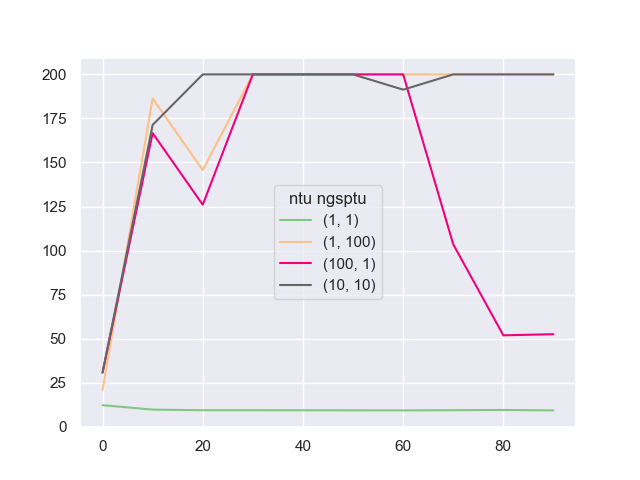
\includegraphics[width=0.5\linewidth]{figures/q4.png}
    \caption{Actor-Critic on CartPole. This indicates that using slow target update is important for stable learning, but it doesn't have to be too large. Intuitively, more gradient update is always helpful.}
    \label{fig:q4}
\end{figure}

Please see Figure~\ref{fig:q4}. Takeaway: using slow target update is important for stable learning, but it doesn't have to be too large. Intuitively, more gradient update is always helpful.
